\begin{center}
    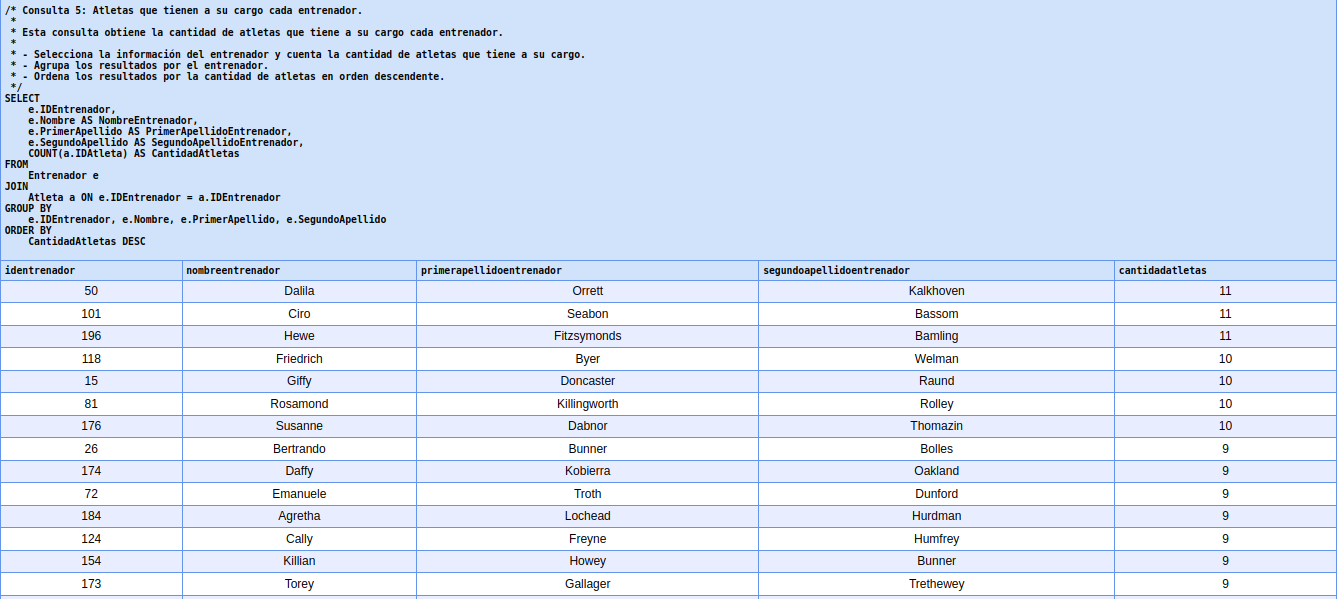
\includegraphics[width=16.5cm]{../resources/Chapters/Consultas/Imagenes/Consulta5.png} 
    
   Consulta 5. Atletas que tienen a su cargo cada entrenador. 
\end{center}

\textbf{Propósito de la consulta}

La consulta tiene como objetivo obtener un listado de entrenadores junto con la cantidad de atletas que tienen a su cargo. Esto es útil para entender la distribución de atletas entre los entrenadores y detectar posibles desequilibrios en la asignación de recursos.

\textbf{Desglose de la consulta}

\begin{itemize}
   \item \textbf{Selección de columnas (\texttt{SELECT})}:
   \begin{itemize}
       \item Se seleccionan las siguientes columnas del entrenador:
       \begin{itemize}
           \item \texttt{e.IDEntrenador}: Identificador único del entrenador.
           \item \texttt{e.Nombre}: Nombre del entrenador.
           \item \texttt{e.PrimerApellido}: Primer apellido del entrenador.
           \item \texttt{e.SegundoApellido}: Segundo apellido del entrenador.
       \end{itemize}
       \item Se utiliza la función agregada \texttt{COUNT(a.IDAtleta)} para contar cuántos atletas están asociados con cada entrenador. Esta columna se denomina \texttt{CantidadAtletas}.
   \end{itemize}
   
   \item \textbf{Tablas involucradas (\texttt{FROM} y \texttt{JOIN})}:
   \begin{itemize}
       \item La consulta utiliza dos tablas:
       \begin{itemize}
           \item \texttt{Entrenador (e)}: Contiene la información de los entrenadores.
           \item \texttt{Atleta (a)}: Contiene la información de los atletas.
       \end{itemize}
       \item Se realiza un \texttt{JOIN} entre ambas tablas utilizando la relación \texttt{e.IDEntrenador = a.IDEntrenador}. Esto asegura que solo se consideren los atletas que están asignados a un entrenador.
   \end{itemize}
   
   \item \textbf{Agrupación de resultados (\texttt{GROUP BY})}:
   \begin{itemize}
       \item Para calcular la cantidad de atletas por entrenador, se agrupan los datos según las columnas únicas del entrenador:
       \begin{itemize}
           \item \texttt{e.IDEntrenador}, \texttt{e.Nombre}, \texttt{e.PrimerApellido}, \texttt{e.SegundoApellido}.
       \end{itemize}
       \item Esto garantiza que se genere un registro único por cada entrenador.
   \end{itemize}
   
   \item \textbf{Ordenamiento de resultados (\texttt{ORDER BY})}:
   \begin{itemize}
       \item Los resultados se ordenan por la columna \texttt{CantidadAtletas} en orden descendente (\texttt{DESC}), de modo que los entrenadores con más atletas aparezcan primero.
   \end{itemize}
\end{itemize}

\textbf{Análisis detallado}

\begin{enumerate}
   \item \textbf{Relación entre tablas:}
   \begin{itemize}
       \item La consulta asume que existe una relación directa entre las tablas \texttt{Entrenador} y \texttt{Atleta} a través de la clave foránea \texttt{a.IDEntrenador}, que apunta a \texttt{e.IDEntrenador}.
       \item Esto implica que:
       \begin{itemize}
           \item Cada atleta tiene asignado exactamente un entrenador.
           \item Un entrenador puede tener asignados uno o más atletas.
       \end{itemize}
   \end{itemize}
   
   \item \textbf{Uso de la función agregada \texttt{COUNT}:}
   \begin{itemize}
       \item La función \texttt{COUNT(a.IDAtleta)} cuenta el número de registros en la tabla \texttt{Atleta} que están relacionados con cada entrenador.
       \item Si un entrenador no tiene atletas asignados, no aparecerá en los resultados porque el \texttt{JOIN} elimina las filas sin coincidencias.
   \end{itemize}
   
   \item \textbf{Agrupación por entrenador:}
   \begin{itemize}
       \item El uso de \texttt{GROUP BY} permite agrupar los registros por entrenador, asegurando que la cantidad de atletas se calcule correctamente para cada uno.
   \end{itemize}
   
   \item \textbf{Ordenamiento:}
   \begin{itemize}
       \item El orden descendente por \texttt{CantidadAtletas} facilita la identificación de los entrenadores con mayor carga de trabajo.
   \end{itemize}
\end{enumerate}

\textbf{Consideraciones}

\begin{itemize}
   
   \item \textbf{Empates en la cantidad de atletas:}
   \begin{itemize}
       \item Si varios entrenadores tienen la misma cantidad de atletas, el orden relativo entre ellos no está definido. Para resolver esto, se podría agregar un criterio adicional en el \texttt{ORDER BY}, como el nombre del entrenador.
   \end{itemize}
\end{itemize}
